\documentclass{standalone}
\usepackage{tikz}
\begin{document}
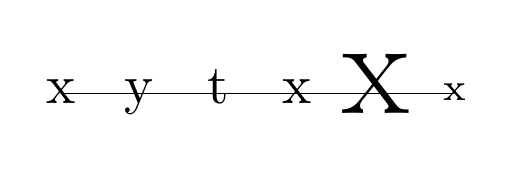
\begin{tikzpicture}[scale=2,transform shape] 
\coordinate (n1) at (0.000,0.000);
\coordinate (n2) at (0.500,0.000);
\coordinate (n3) at (1.000,0.000);
\coordinate (n4) at (1.500,0.000);
\coordinate (n5) at (2.000,0.000);
\coordinate (n6) at (2.500,0.000);
\draw [very thin] (n1) -- (n6);
\node [text height=0.223cm,text depth=0.089cm] 
    at (n1) {x};
\node [text height=0.223cm,text depth=0.089cm] 
    at (n2) {y};
\node [text height=0.223cm,text depth=0.089cm] 
    at (n3) {t};
\node [text height=0.223cm,text depth=0.089cm] 
    at (n4) {x};
\node [font=\Huge,text height=0.428cm,
    text depth=0.171cm] at (n5) {x};
\node [font=\scriptsize,text height=0.149cm,
    text depth=0.059cm] at (n6) {x};
\end{tikzpicture}
\end{document}
